\section{Shape Systematics}
\label{appendix:shapeNPs}


\begin{figure}[htp]
     \begin{center}

        \subfigure[]{%
            \label{fig:mvis}
            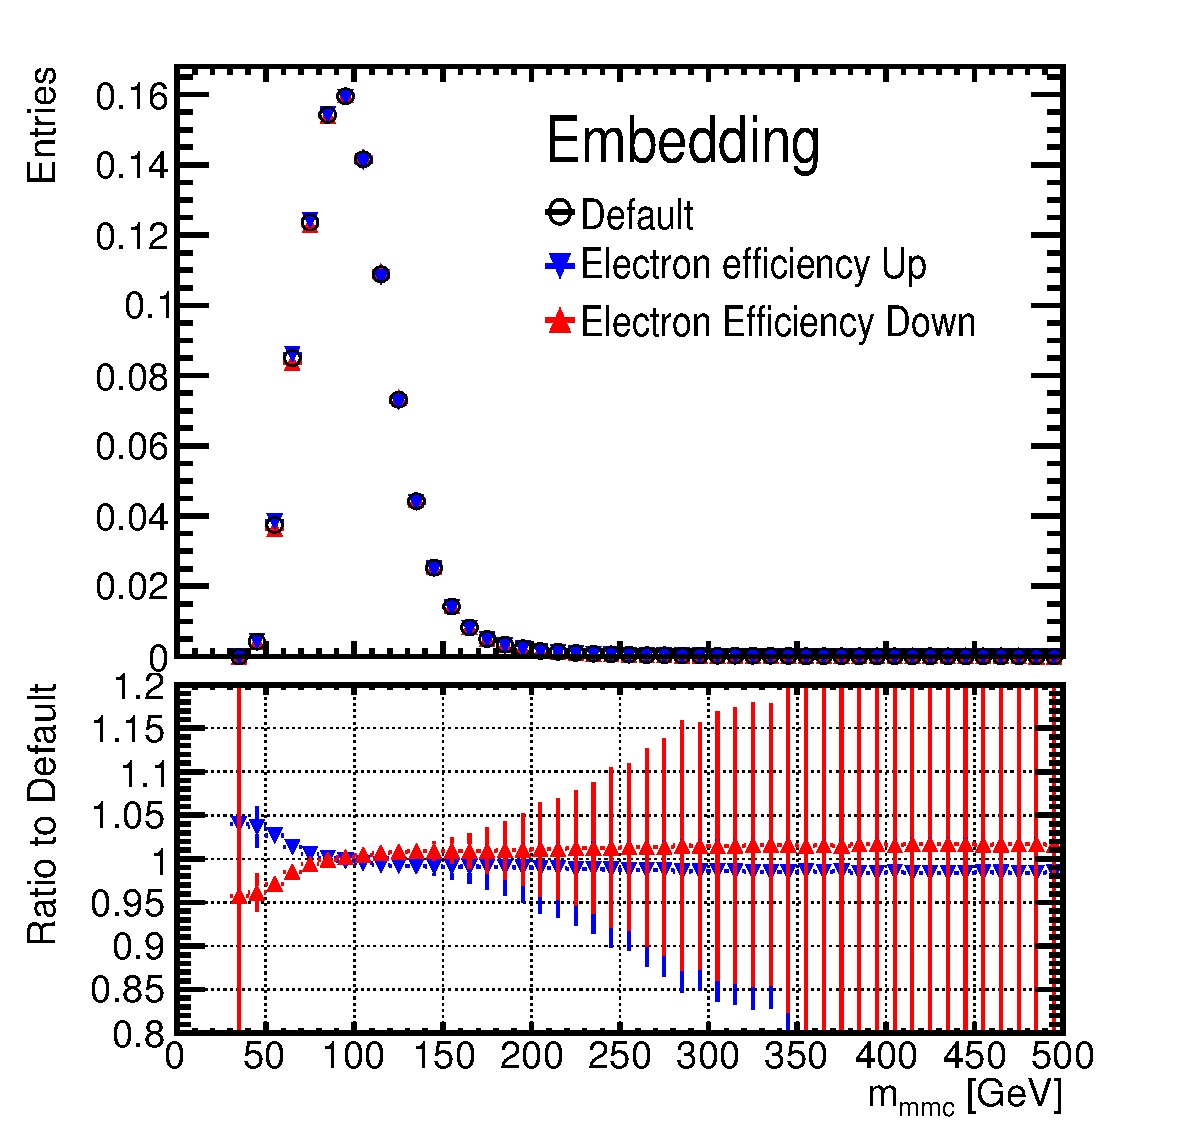
\includegraphics[width=0.45\textwidth]{figure/distributions/NP_Shape_ElecSF_BVeto_mmc.pdf}
	}
	
        \subfigure[]{%
            \label{fig:mmc}
            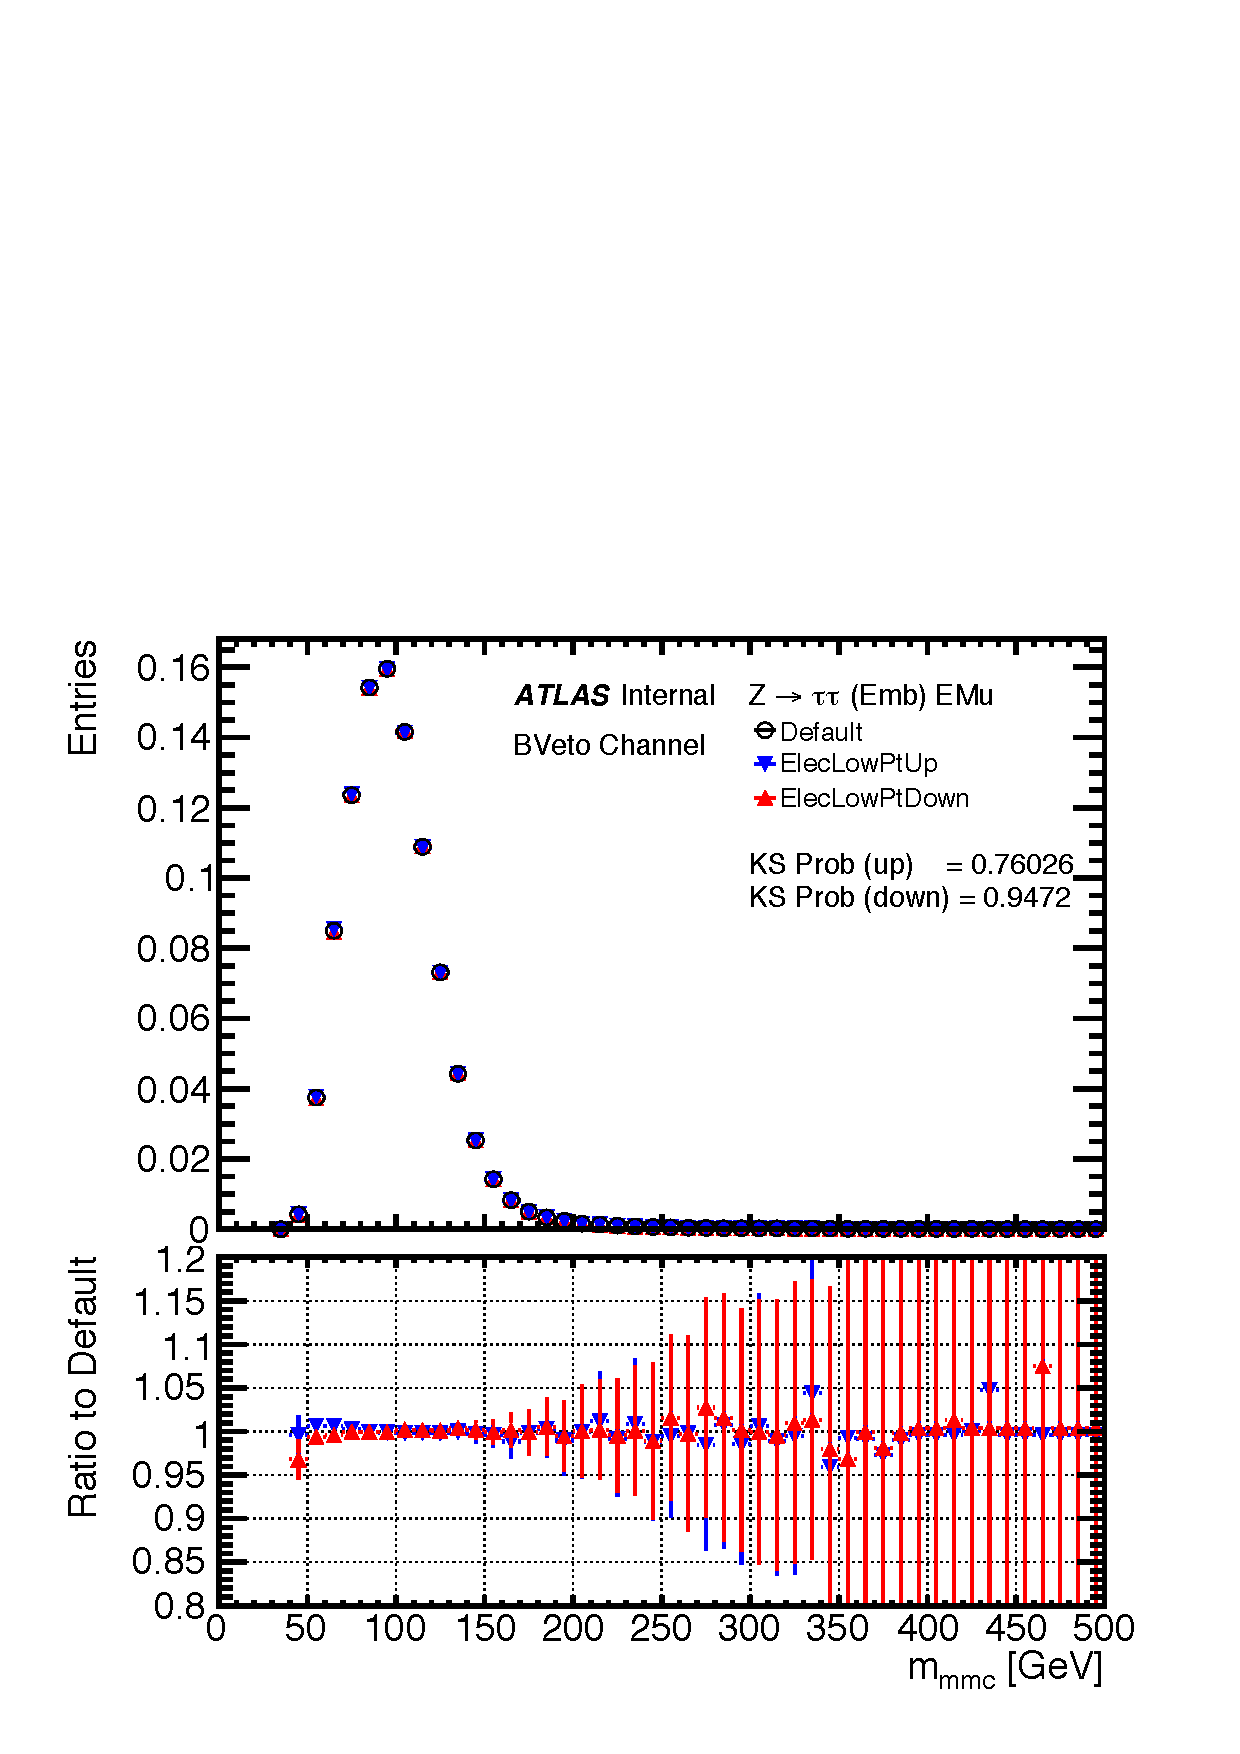
\includegraphics[width=0.45\textwidth]{figure/distributions/NP_Shape_ElecLowPt_BVeto_mmc.pdf}
	}

        \subfigure[]{%
            \label{fig:mmc}
            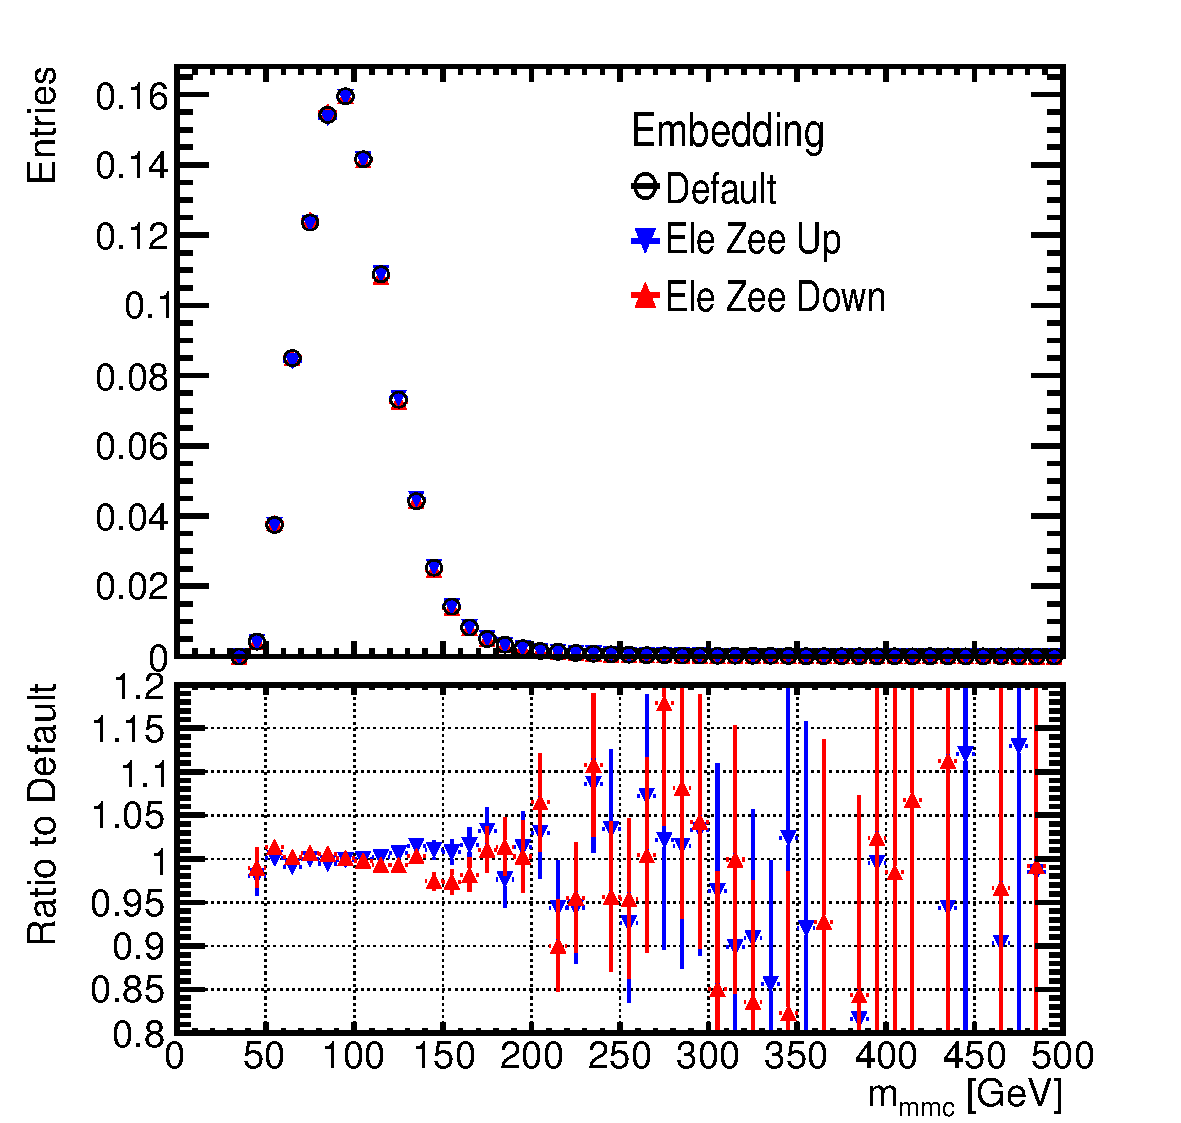
\includegraphics[width=0.45\textwidth]{figure/distributions/NP_Shape_ElecZee_BVeto_mmc.pdf}
	}

    \end{center}
    \caption{Effect on the \mmc distribution of the embedding sample due to the (a) the electron reconstruction and identification systematics, (b) the electron low \pt~ energy scale systematic and (c) the electron Zee energy scale systematic. The plots are made after the full b-veto category selection.}
   \label{fig:ElecShapeNPs}
\end{figure}
